\documentclass[conference, a4paper, 10pt, twocolumn]{IEEEtran}
\usepackage{amsmath,amssymb,amsfonts}
\usepackage{algorithmic}
\usepackage{graphicx}
\usepackage{textcomp}
\usepackage{xcolor}
\usepackage{acronym}
\usepackage{subcaption}
\usepackage[style=ieee]{biblatex}
\usepackage[nottoc]{tocbibind}
\def\BibTeX{{\rm B\kern-.05em{\sc i\kern-.025em b}\kern-.08em
    T\kern-.1667em\lower.7ex\hbox{E}\kern-.125emX}}

\addbibresource{literature_list.bib}
\renewcommand*{\bibfont}{\small}

\newacro{API} {\textit{Application Programming Interface}}
\newacro{UI} {\textit{User Interface}}

\begin{document}

\title{Mechanisms to Raise Awareness about Smartwatch Data Collection}

\author{
	\IEEEauthorblockN{
		Mehmed Mustafa
	}
	\IEEEauthorblockA{
		\textit{Institute of Computer Science}\\
		\textit{University of G\"{o}ttingen}\\
		G\"{o}ttingen, Germany\\
		Email: mehmed.mustafa@stud.uni-goettingen.de
	}
	\and
	\IEEEauthorblockN{
		Chris Warin
	}
	\IEEEauthorblockA{
		\textit{Institute of Computer Science}\\
		\textit{University of G\"{o}ttingen}\\
		G\"{o}ttingen, Germany\\
		Email: chris.warin@stud.uni-goettingen.de
	}
}

\maketitle
\thispagestyle{plain}
\pagestyle{plain}


\begin{abstract}
This document is a model and instructions for \LaTeX.
This and the IEEEtran.cls file define the components of your paper [title, text, heads, etc.]. *CRITICAL: Do Not Use Symbols, Special Characters, Footnotes, 
or Math in Paper Title or Abstract.
\end{abstract}

\begin{IEEEkeywords}
smartwatch, awareness, feedback, sensor, privacy
\end{IEEEkeywords}

\section{Introduction}
The well-known privacy-paradox \cite{williams2019smart,patil2015interrupt} is prevalent in smartwatches: users are concerned about the pervasiveness of ubiquitous devices such as smartwatches, but they also have misunderstandings, or even false beliefs concerning these devices \cite{udoh2016privacy}. This points at the importance of raising awareness in smartwatch data collection, as users need to understand what, how, and when their data is collected by the sensors of their watch, in order to better protect their privacy. 

The emerging question to this problem is: how do we raise user awareness on smartwatch data collection? Where past contributions have used serious games as an approach \cite{williams2019smart}, we implemented different types of feedback in an application that randomly collects sensor data in order to show users that their data is being collected in real-time. Our solution lets users choose between different visual, haptic and sonor configuration which provide a good granularity of feedback, thus matching different profiles. Moreover, we provide users with control on data collection by supporting a sensor suspension mechanism through a timer. The architecture of the project is split between a watch face (i.e. an application that acts as the main interface for the user which displays time among other things) and a main application that accesses sensors and forwards feedback messages to the watch face. This makes for an easy sharing of the watch face that can then be easily connected by a developer to their own application, if they wanted to facilitate transparency.

The structure for this report is as follows: the necessary terms and concepts to understand our work are described in section \ref{foundations}. Then, we analyse contributions in the domains of privacy concerns and smartwatch feedback separately before looking at works that include both of these domains together in section \ref{related}. A description of our approach is detailed in section \ref{approach}. We then discuss the advantages and limits of this solution in section \ref{discussion}, along with results regarding our first approach on this topic. Finally, we conclude this work in section \ref{conclusion}.   

\section{Foundations}\label{foundations}

The main goal of our work is to raise the awareness about smartwatch data collection. In this section, we first clarify our notion of smartwatch data collection and describe the technologies and platforms we use. 

A smartwatch is a device in the form of a watch which has computing capabilities. Although the earlier models had restricted functionality, the models starting from early 2010s are closer to smartphones in regard to features. Modern smartwatches have WiFi/Bluetooth connectivity, support mobile apps, have their own operating system and peripheral devices, which may include health tracking sensors such as heart rate monitors, location tracking sensors such as GPS receivers and activity tracking sensors such as pedometers.\cite{smartwatch}

Mobile apps may gather data from different sensors at any given time. We refer to this process as smartwatch data collection. Mobile apps often ask the permission to use different sensors when they are launched for the first time. Users give permission but are not aware of exactly when and how often apps gather, e.g., their health, location or activity data. We propose 3 different mechanisms to increase the awareness users about the data gathering process: Visual, Sound and Haptic feedback. The visual feedback divides into 3 sub categories: Ring, Icon and Notification. The awareness increasing mechanisms are discussed in more details in section \ref{approach}. Our proposal could be further extended and developed as an API which developers could use in the future.

\begin{figure}[t]
\leftline{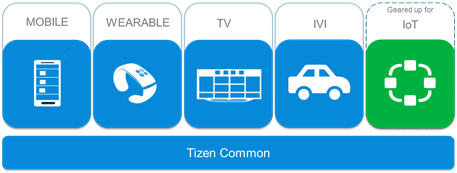
\includegraphics[width=.5\textwidth]{img/tizenInfrastructure.png}}
\caption{Tizen infrastructure~\cite{tizen}}
\label{fig:tizen}
\end{figure}

For our research, we used a Samsung Galaxy Watch 3 \cite{galaxyWatch3}. The smartwatch runs Tizen OS 5.5, an open source Linux-based mobile operating system which is built to work on diverse devices. In order to support different types of devices and provide product-optimized performance, Tizen uses different profiles to categorize functions and features according to the requirements of each device type. Currently, four profiles are supported: IoT, Mobile, TV, and Wearable. Since all profiles are built on top of a common, shared infrastructure (as shown in Fig.~\ref{fig:tizen}), it is easy to add new profiles for emerging technologies \cite{tizen}.

Tizen has its own official IDE for developing web based and native applications. Moreover, the availability of Tizen extensions for the Visual Studio Family makes possible to develop Tizen applications in the .NET environment. Tizen .NET, in comparison to web and native frameworks, is more advantageous. The C-based framework does not have advantages of a managed runtime and the HTML5-based framework has fewer features supported and worse performance. On the other hand, Tizen .NET has managed runtime advantages such as faster development, safer code, cross-platform support and better quality software. Tizen provides an emulator which increases the application development process. Firstly, because we do not need an actual physical device to start the development process. And secondly, because the control panel of the emulator makes it possible to produce different sensor values \cite{tizen}.

It is, however, important to note that Tizen .NET relies on various components from different entities: the .NET framework \cite{dotnet} is maintained by Microsoft, as well as the cross-platform \ac{UI} framework Xamarin.Forms \cite{xamarin}. On top of this comes CircularUI \cite{circularUI}, which is maintained by Samsung and extends Xamarin.Forms for Samsung-specific hardware. Lastly, in a similar fashion, Samsung extends the .NET \ac{API} with TizenFX \cite{tizenFX} for hardware specific methods that are not covered by the base framework.

\section{Related Work}\label{related}
Our topic englobes two distinct domains. First, raising awareness about smartwatch data collection is important because users have both privacy concerns and misconceptions about smartwatches. This is pointed out by Datta, Namin and Chatterjee: in their survey of the literature in the field of privacy concerns in wearable devices, they identify that user concerns vary depending on the context \cite{datta2018survey}. For example, users were more concerned if there was a spacial context in the data, because they understood their position could be inferred. The same conclusion is drawn by Motti and Caine: they claim that users see the GPS sensor in wrist-mounted devices as the most critical privacy concern \cite{motti2015users}. Moreover, Udoh and Alkharashi reveal that participants in their study held wrong beliefs when it came to privacy and wearables \cite{udoh2016privacy}. This confirms the importance of raising awareness by providing clear, understandable information about data collection. These studies, however, only analyse the concerns of users without proposing mechanisms to raise awareness.

Secondly, the topic implies that to raise awareness, there is a need to attract the attention of users when their smartwatch collects their data through the sensors. In other words, feedback needs to be given to users in such cases. There has been a plethora of proposals of feedback for various situations in the last years. In \cite{dobbelstein2016unconstrained}, they propose a system based on haptic feedback to help pedestrians to navigate to their objective. The authors of \cite{goodman2020evaluating} propose a solution to assist deaf people by giving them visual and haptic feedback related to their sonor environment. In \cite{lee2019smartwatch}, they implement a system that gives chest-compression feedback to assist rescuers in performing cardiopulmonary resuscitation. These proposals show the potential of feedback in various situations in the sense that it can easily attract the attention of the user to give them important information. As such, it can be a viable mechanism that can be used to raise awareness related to wearable data collection.

It is observable that despite the high amount of contributions in both analyses of user privacy concerns and unawareness, and applications that give feedback for various contexts, there is, to the best of our knowledge, little work that merges both domains together. Patil et al. assess the importance of privacy feedback and question the impact of its timing on user experience, arguing for a moderate delay \cite{patil2015interrupt}.  Although our implementation provides real-time feedback, we still consider it a viable approach as the provided feedback is never blocking the user. A recent contribution from Williams, Nurse and Creese evaluates the efficiency of serious games in encouraging privacy-protective behaviour, claiming to be the first tool for this matter \cite{williams2019smart}. While this encouraging approach seems to raise privacy awareness in smartwatch users, it differs from ours in the sense that it uses a game rather than real-time feedback. In other words, there is seemingly no system that focuses on raising awareness of users regarding smartwatch data collection through real-time feedback.  

\section{Approach}\label{approach}

\subsection{System requirements}

\subsubsection{Functional requirements}
\subsubsection{User interface requirements}
\subsubsection{Security and privacy requirements}

\subsection{System overview}

% System overview
\begin{figure*}[ht]
\centerline{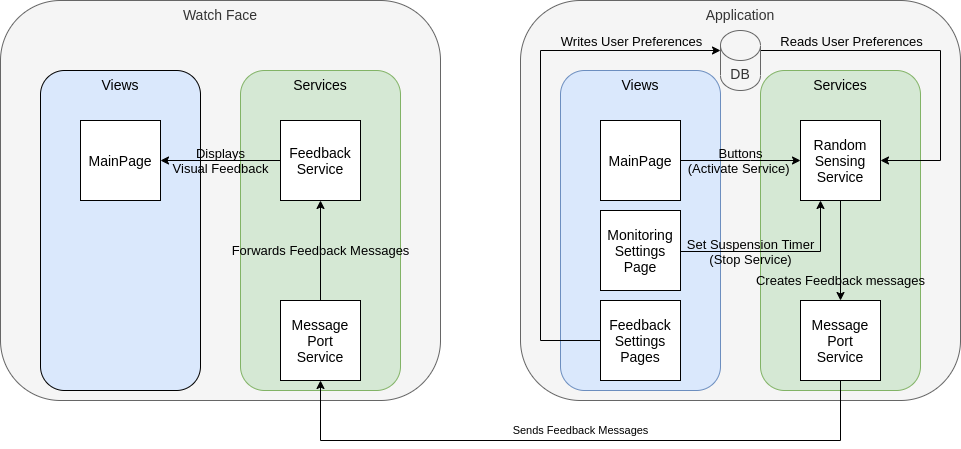
\includegraphics[width=.9\textwidth]{img/appDiagram.png}}
\caption{System overview}
\label{fig:systemOverview}
\end{figure*}

Fig.~\ref{fig:systemOverview} illustrates the system overview. We have developed two applications: main and watch face. The main application is responsible for: 1) applying feedback and monitoring settings defined by the user and storing them on the device, 2) simulating random sensor accesses by using the random sensing service and generate matching feedback data, and 3) sending the feedback data to the watch face application via the message port service. The watch face application, on the other hand, is responsible for: 1) receiving feedback data from the main application via the message port service and 2) transforming the feedback data into actual feedbacks and notifying the user about the collected sensor data according to their feedback preferences.

\subsection{Services}\label{services}
The main logic of the applications is controlled by several services.

\subsubsection{Human activity services}
Our design covers three types of human activity services: 1) Health service, 2) Location service, and 3) Activity service. These three services cover the basic and generic sensors.

The health service has an instance of the smartwatch's heart rate monitor sensor. This sensor returns beats-per-minute (between 0-220) data in a given interval of time (between 0-5000 ms).

The location service supports four different location positioning system types: 1) Gps, which uses the global positioning system, 2) Wps, which uses the Wi-Fi positioning system, 3) Passive, which uses the passive mode, and 4) Hybrid, which selects the best method available at the moment. 

The activity service could potentially have an instance of the podometer sensor. However, this functionality was not implemented. Nevertheless, we still consider cases which may involve activation of the activity service and handle them accordingly by showing the appropriate feedback to the user. 

\subsubsection{Privacy permission service}
The privacy permission service is responsible for checking privacy-related privileges and requesting permission from the user to use specific privileges. For example, in order to use the heart rate monitor sensor, an application must first request and get the health privilege from the user. In the same way, the location privilege must be requested and obtained first in order to allow the usage of the location service.

\subsubsection{Random sensing service}
The random sensing service is responsible for the creation of random sensor accesses. This service is not required in a real-life scenario application because the sensor accesses would occur in a logical context (e.g. at a certain time of the day). In our research, we have to simulate such sensor accesses. This service starts and stops human activity services. Four different actions are supported: 1) Start one random service, 2) Start the maximum amount of random services (2 in our work), 3) Stop one random service, and 4) Stop all services. A random action takes place every few seconds (5 seconds in our case).

Although the name suggests that this service randomly manipulates the activity of the human activity services, this process is not completely random. In order to make smart and efficient choices, it is required to take into consideration two factors: 1) current activity of the services and 2) previously generated random action. It makes no sense to try to activate a service which is already active or to deactivate one which is not active. It also makes no sense to perform action 1) or 2) if the current amount of active services is already the maximum amount, or to perform action 3) or 4) if there are currently no active services. Taking these 2 factors into consideration guarantees that a different feedback will be triggered on the watch every time a random action is generated.

\subsubsection{Message port service}
The message port service is responsible for the communication between the two applications. In our design, we use uni-directional message port communication. In other words, we use a single port on each application to send and receive data, since we need a one way communication---from the local port of the main application sending feedback data to the remote port of the watch face application. The received feedback data is then forwarded to the feedback service.

\subsubsection{Feedback service}
The feedback service is responsible for the transformation of the received feedback data (active services and user settings) into actual feedback parameters (visualization feedback type, color and activity status of other/additional feedback types) and triggering the feedbacks on the watch face application's main page. 


\subsection{Supported feedback types}

% Visual Feedback images
\begin{figure*}[t!]
    \centering
    \begin{subfigure}[t]{0.33\textwidth}
        \centering
        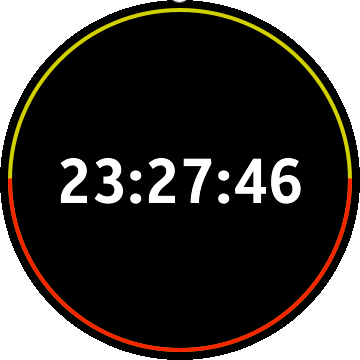
\includegraphics[height=1.5in]{img/ringHR&Location.png}
        \caption{Ring - HR and Location}
        \label{fig:ringFeedback}
    \end{subfigure}%
    \begin{subfigure}[t]{0.33\textwidth}
        \centering
        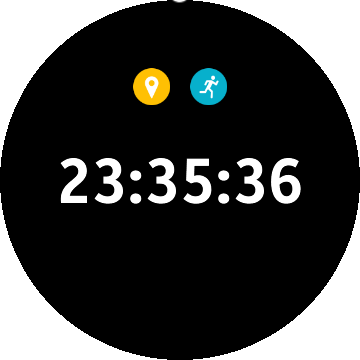
\includegraphics[height=1.5in]{img/iconLocation&Activity.png}
        \caption{Icon - Location and Activity}
        \label{fig:iconFeedback}
    \end{subfigure}
    \begin{subfigure}[t]{0.33\textwidth}
        \centering
        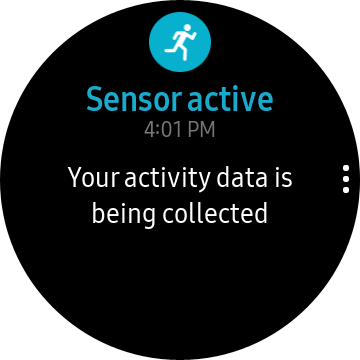
\includegraphics[height=1.5in]{img/notificationActifity.png}
        \caption{Notification - Activity}
        \label{fig:notificationFeedback}
    \end{subfigure}
    \caption{Different kinds of visual feedback}
    \label{fig:visualFeedbackImage}
\end{figure*}

We divide the supported feedback types into two main groups: 1) Visual feedbacks and 2) Other feedbacks.

\subsubsection{Visual feedbacks}
We assign three colors---red, yellow and blue---for the main three human activity services: health, location and activity, respectively.

The visual feedbacks are further categorized into there sub groups: 1) Ring feedback, 2) Icon feedback, and 3) Notification feedback (as shown in Fig.~\ref{fig:ringFeedback},~\ref{fig:iconFeedback}, and~\ref{fig:notificationFeedback}, respectively).

\textbf{Ring feedback}: this feedback type draws a slowly blinking ring around the screen of the watch, by using the progress bar feature of the device. The color of the ring depends on the currently active services. In case there are two active services at the same time, the ring is divided into two equal parts and each part has the color of the respective active service. Fig.~\ref{fig:ringFeedback} shows an example of the ring feedback type when both health and location services are active. For our research, and for the sake of keeping the implementation simple, the maximum amount of active services at the same time is set to two. Since we use the progress bar feature to achieve the ring feedback, it is enough to assign one color for the progress bar and another color for the progress bar's background, and make the value of the progress bar 0.5 to split it into two equal parts. Theoretically, it is possible to have more than two active services at the same time. However, in a such scenario the blinking ring would be divided into more equal parts, and hence, a more complex algorithm would be needed. 

\textbf{Icon feedback}: this feedback type shows an icon according to which service is active. The icons follow the same color pattern(i.e. the health service has a red color, and so on). Fig.~\ref{fig:iconFeedback} shows an example of the icon feedback type when both location and activity services are active. In comparison to the ring feedback, the icon feedback is a lot more easier to implement in case there are more than two services active at the same time. This is because we used a FlexLayout (a Xamarin.Forms component) in order to correctly center icons regardless of their amount. Hence, the number of the active services does not matter. There is however a maximum limit, which is defined by the screen area.

\textbf{Notification feedback}: this feedback type, as its name suggests, shows a system notification with a title and a message. The messages are of the type: ``Your <health/location/activity> data is being collected'', with according singular or plural grammar depending on the case. If there is only one active service, an icon is additionally shown. When more than one service is active, the generated notification does not show any icons, because Tizen notifications only support one icon. This feedback type gets more suitable as the number of the active services increase, because the message can easily convey the list of active sensors without taking too much space.

\subsubsection{Other feedback types}
The other feedback types are: 1) Vibration and 2) Sound. These two feedback types are additional feedback and could be considered as an extension to the visual feedbacks, in the sense that they can be added on top of the visual feedbacks (they are deactivated by default). The user may combine one of the visual feedbacks with vibration and/or sound according to their preference from the settings menu, to the exception of the notification type, for which vibration and sound depend on the global system settings---this is to avoid having two sounds and two vibrations at the same time. We do not consider different vibration intensities or sound types; however, they differ from the system notifications' sound and vibration, which are defined in the system settings. Although the system notifications' sound and vibration intensity can be adjusted to a low level in the watch's settings, our own vibration intensity and sound have been designed to be less intense than the system notification ones.

\subsection{Main application}
The main application's user interface is designed to be simple to use and to not overwhelm the user with options. We used the Shell system from Xamarin.Forms to create routes to the different pages in a way that lets the user navigate easily between them. This is done by using so-called ``flyout'' items, which are accessible by clicking a small arrow at the botom of the screen. Clicking this arrow shows a dropdown list on top of the current page, which shows the available pages.

The main page has a single button which activates and deactivates the random sensing service (the service is discussed in details in section \ref{services}). It exists mainly for testing purposes and could be removed in the future.

The feedback settings page consists of two sub pages, that are navigable by swipe gestures: visual feedback settings and other feedback settings. In the visual feedback settings page, the user can select one of the three available options: 1) Ring, 2) Icon, and 3) Notification (as shown in Fig.~\ref{fig:visualFeedbackSettings}). The radio buttons convey that only one choice is possible. In the other feedback settings page, the user can select additional feedback options such as vibration and sound (as shown in Fig.~\ref{fig:otherFeedbackSettings}) Here, switches communicate that these options can be combined.

In the monitoring settings page, the user can suspend the application's sensor usage for a defined amount of time, as shown in Fig.~\ref{fig:monitoringSettings}. During that time interval, the main application, or more specifically the random sensing service, is not permitted to read any sensor data. 


% Feedback Settings images
\begin{figure*}[t!]
    \centering
    \begin{subfigure}[t]{0.32\textwidth}
        \centering
        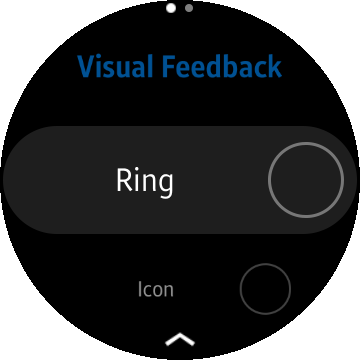
\includegraphics[height=1.5in]{img/settingsVisualFeedback.png}
        \caption{Visual feedback settings}
        \label{fig:visualFeedbackSettings}
    \end{subfigure}%
    \begin{subfigure}[t]{0.32\textwidth}
        \centering
        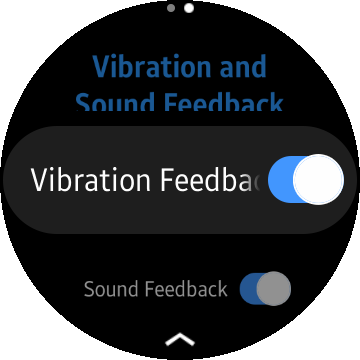
\includegraphics[height=1.5in]{img/settingsOtherFeedback.png}
        \caption{Other feedback settings}
        \label{fig:otherFeedbackSettings}
    \end{subfigure}
    \begin{subfigure}[t]{0.32\textwidth}
        \centering
        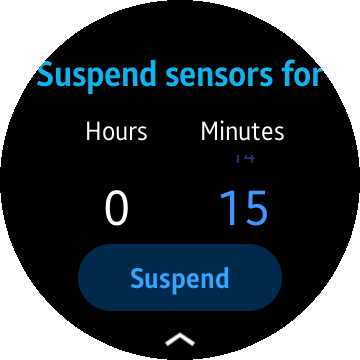
\includegraphics[height=1.5in]{img/settingsSuspend.png}
        \caption{Monitoring settings}
        \label{fig:monitoringSettings}
    \end{subfigure}
    \caption{Feedback and monitoring settings}
    \label{fig:feedbackSettingsImage}
\end{figure*}


\subsection{Watch face application}
The watch face application is, for research and design purposes, very minimalistic. By default, it only shows the current time digitally. When the main page receives feedback instructions from the feedback service, the necessary visual components are dynamically parametered and made visible. In case of the ring feedback, the progress bar values and colors are adapted and made visible. In case of the icon feedback, the respective icons are made visible. Lastly, in case of the notification feedback, nothing is made to the level of the main page, as the system notification naturally triggers and takes the space of the screen, in case the watch face is active. In case not (e.g. the user is using another application), then the notification only pops up at the top of the screen for a few seconds, before disappearing to the notification center. 

When the user activates the ``always on'' mode of their smartwatch, the ambiant mode can be triggered. This happens when no interaction is made after a few seconds. When the screen would normally turn off, the ambiant mode instead reduces the luminosity and the amount of \ac{UI} updates. This permits users to still see the time when the watch's screen should be off. In order to save resources, the ring feedback's blinking animation is suspended in this mode, but the color and value of the progress bar are still updated in real time, in order to keep the fedback accuracy in relation to the sensors that are accessed by the main application.

\section{Discussion}\label{discussion}
This section discusses the different approaches that were used in order to raise awareness in smartwatch data collection. Prior to developping the application that was discussed in section \ref{approach}, we imagined another application that was, to the best of our knowledge, not realizable with current \acp{API} and system accesses.  

\subsection{First approach}
The first application that we attempted to develop relied on a monitoring mechanism that would detect any sensor usage by another application that is installed on the watch. This way, the application would have been able to alert the user when an application that they chose to monitor would have started sensing. Unfortunately, this approach was impossible to implement, although the necessary data for its functioning are existing.

In order to implement the mechanism, three pieces of information would have been necessary: 1) the time at which a sensor was accessed by an application, 2) the name of the requested sensor, and 3) the process ID of the application that requested the sensor. We thought about two possible ways of obtaining this information: first, through the .NET Standard \ac{API} - and by extention, Samsung's .NET \ac{API} that contains platform-specific functionalities\cite{tizen}. However, upon a thorough inspection of the documentation, we came to the conclusion that these \acp{API} do not provide methods to access sensors in a global context. This means that although it is possible to create instances of the \textbf{Sensor} class, these instances are only related to the context of the application. In other words, it is only possible to know whether a sensor is being accessed by the current application, but not by others. 

The second way to obtain the necessary information was to read the system log. This log contains all necessary data; as such, parsing it would allow the application to detect when a certain application reads a given sensor. Unfortunately, this idea also led to a dead end: although the system log is writable by any application, it is not made readable by the vendor. This is certainly for a security reason, as an application that can both read and write the log could impersonate another application. Currently, the log is only readable through the development bridge that is provided by Tizen. As such, the only way to read the log of a smartwatch is to have a nearby computer with the required tools, which made our implementation impossible for a standalone application on a smartwatch. An alternative to this would be gaining root access to access the log from the smartwatch, in a similar fashion as on Android devices. However, there are, to this day, no accessible ways to achieve this. Furthermore, even if there were, this would result in a non-accessible application, as we assume that most smartwatch users would not go through the hassle of rooting their device, especially not to obtain feedback about sensor usage. 

%Lack of Tizen documentation details - app_context_h - structure data -> not possible to peek and see what is this abstract data structure constructed from - in Native app

These dead-ends point at the lack of sensor data access, and eventually, at feedback mechanisms by smartwatch vendors and the Tizen platform. The only sensor related feedback offered by the smartwatch we used for development (Samsung Galaxy Watch 3) is the green light that blinks when the heart rate monitor is turned on---and it is not even a voluntary feedback given by the vendor, but a necessary light to calculate the heart rate of the user. Although it would be best if smartwatch vendors provided native mechanisms to raise awareness in sensor data collection, a good start would be for them to extend their \acp{API} in order to know if sensors are used by other applications. This would allow the development of applications similar to our first approach that could seduce users. As of today, we come to the conclusion that smartwatch application developers have to implement these mechanisms themselves like we did in our second approach.

\subsection{Second approach}
The impossibility to implement our first approach led us to start again from scratch, and develop the application described in section \ref{approach}. Although it is less generic than our first approach---in the sense that it can only give feedback related to sensors that it senses itself---it still offers functionalities that benefit users, but also potentially developers that want to create transparent applications regarding sensor data collection.

Firstly, our main application provides a good granularity of feedback for the user, in the sense that the three different types of visual feedback that the user can choose attract attention with a different intensity: the icons are more discreet than the blinking rings, which are in turn more discreet than the system notifications, which attract the most attention with a colorful cue, a long vibration and a loud sound. This can further be tuned with options to add vibration, sound, or both to the ring or icon visual feedbacks (the notification type already comes with its own sound and vibration). As a result, different combinations can be made to obtain various amounts and intensities of feedback, which can suit different kinds of users. For example, users that are interested in knowing when their smartwatch sensors are being used by the application but do not want to be constantly reminded can use the ring or icon visual feedback types without sound or vibration. This way, they will only notice sensor usage when they look at their watch and see visual feedback on the watch face. Similarly, users who want more knowledge and control on sensor usage can either use the notification feedback type, or add vibration and sound to the ring or icon visual feedback types. Adding sound or vibrations provides more active feedback as they attract the user's attention even when they are not looking at their smartwatch. 

Secondly, the sensor suspension mechanism empowers the user by letting them choose when and for how long the application will not read sensor data. Along with providing them control, this can also reassure them regarding transparency: they know that the application will not collect their personal data as they will not get any feedback. Furthermore, the empowering of users in this matter can also come from the previously mentioned granularity of feedback, as the users can adjust the amount and intensity of feedback to their liking. Gaining control over the collection and having choice over the feedback can put the user in a position where they no longer feel overwhelmed by the pervasiveness of technology.

% see if this can be tied to human in the loop lecture from usable security - a ref would be great as this is only assumptions we do since we have no study to prove our point 

Lastly, the design of our application is advantageous for future work and other developers. Our implementation relies on a communication between the main application, which does the sensing, and a watch face, that displays feedback upon receiving messages from the main application. The communication between the two components is made using the .NET \ac{API}. As a result, it would be possible to release the source code for the watch face component, along with an easy to follow documentation to indicate how to communicate with it. This way, developers could easily reuse the watch face and connect it to their own application.

Although our approach has several advantages, it also has its limits. The first one is that it is a mere prototype, in the sense that it is not a realistic application that could be released on the vendor's store. The application only randomly accesses the smartwatch sensors at random times, which is likely not how a realistic application would behave. This is, however, not an important point when considering how to raise awareness for data collection---the point of this application is rather to consider the efficiency of feedback that is related to sensor data.  

Another limit of this implementation is the application performance: during the development, we found that the smartwatch battery was depleting fastly, implying a heavy resource consumption from our application. This can be improved over time by getting a better understanding of the platform and therefore apply the best practices that the vendor recommends. Indeed, the various components that are part of Tizen .NET (see section \ref{foundations}) imply different documentations, which sometimes contradict each other, or are outdated. This makes it hard to fully understand the Tizen ecosystem and, therefore, to program efficiently for it. However, this limit can also be discarded when considering awareness for sensor data collection.

Lastly, our implementation can easily be bypassed by the user, if they simply chose to close or not run the main application. It would then not access any sensor until the user launched the application again. When considering a real-life case, it is probable that developers would put the sensor access logic in services applications that run in background. This would, however, raise the necessity to ensure that such background services could be stopped when the data they gather is outside the scope of the purpose for which they are collected. For example, if we consider a scenario where a company provides its employees with an internal application that collects sensor data (e.g. to assess the employees' wellness), then such an application should not be allowed to sense data outside of working hours. Such a scenario is discussed by Richter in \cite{richter2020privacy}. Regardless, this limitation is rather related to the platform than the problem of raising awareness. 

Globally, none of the limitations of our current approach are critical when considering mechanisms to raise awareness in smartwatch data collection. However, the impossibility to implement the first one is in itself the major limit that prevented us from going further into this more global direction of providing feedback in a general way for all sensor accesses---not just the current application.

\section{Conclusion}\label{conclusion}
This report presented our proposal for mechanisms that raise awareness about smartwatch data collection. An overview of the capabilities of current smartwatches and their systems is described is section \ref{foundations}. We compared our work with past litterature. On one hand, there is evidence about users' privacy concerns when it comes to smartwatch devices \cite{udoh2016privacy,datta2018survey,motti2015users}. On the other hand, there are various proposal of systems that give feedback to users for various usages, such as medical \cite{lee2019smartwatch}, accessibility \cite{goodman2020evaluating}, or navigation \cite{dobbelstein2016unconstrained}. However, these two fields are, to the best of our knowledge, not connected together. As such, we are not aware of mechanisms that give users real-time feedback related to data collection in smartwatches, with the exception of \cite{williams2019smart}, which raises awareness through the use of a serious game, but not feedback. 

Given this, we attempted to create a monitoring application that could detect when installed applications access sensors, and give feedback accordingly. This attempt resulted in failure, due to the lack of tools to achieve our goal. This result hopefully points out at the necessity for vendors to provide \acp{API} that can indicate sensor usage in a global context instead of restricting it to the app context only. 

From this, we implemented a prototype application that sends various types and combinations of feedback to the user when it accesses smartwartch sensors, including visual, haptic and sonor feedback. The application is divided between a watch face (i.e. the main interface of a smartwatch which mainly displays the time among other things; here, visual feedback) an a main application which accesses sensors and sends messages to the watch face. The main application also supports user preferences: the user can choose between different visual feedbacks and whether they want to add sounds or vibration on top of the visual feedback. These diferent combinations allow for a wide granularity of feedback, which can better suit users depending on the amount of feedback they want. Furthermore, users are put in control through a sensor suspension mechanism: they can set a timer until which the application can not access any sensor. Globally, this approach should both reassure users when they do not perceive any feedback (because this implies no collection of their data) and raise their awareness when the feedback informs them of data colleciton.  

The interest for this project is that it mimicks what a real-life application could do. Considering a scenario where a company provides its employees with an application that collects sensor data in a transparent way (i.e. by giving corresponding feedback) justifies our application in the sense that this could be the next step for smartwatch applications in the future \cite{richter2020privacy}. Furthermore, the watch face code could be shared to the Tizen community as a first step towards a global \ac{API}. As such, having groundwork in this direction is of importance. User tests will need to be conducted in the future in order to assess the efficiency of the provided feedback in relation to raised awareness. 

\section*{Acknowledgment}
The authors would like to thank their supervisor, Alexander Richter, for providing feedback and visual resources, which helped modeling their approach a lot.

\printbibliography

\end{document}
